\subsection{Evidence phases and decision points}
Figure~\ref{fig:workflow} traces a frozen score from its cohort and model to the trials that may set the threshold and the trials on which its decisions are judged.
\begin{figure*}[t]
\centering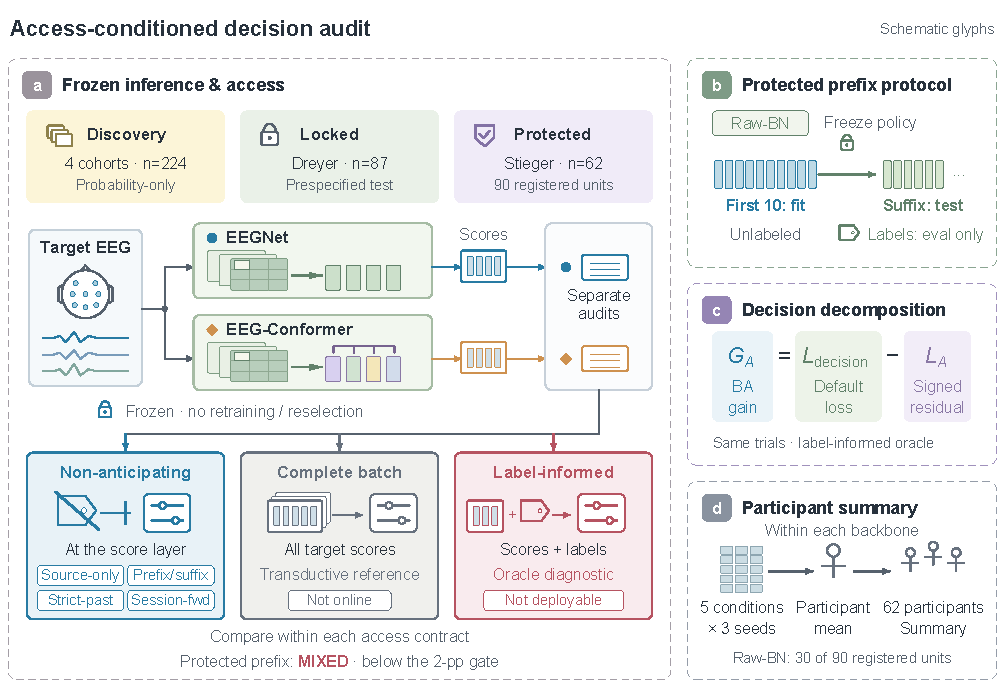
\includegraphics{figures/figure1_acdd_workflow.pdf}
\caption{Decision audit across three evidence phases. (a) Access is specified at the interface of already generated scores. Source-only, fixed-prefix, strict-past and session-forward rules exclude future target scores and target labels from threshold fitting. Complete batch reads future scores. The oracle uses evaluation labels. (b) The protected fit sees the first ten scores and is held fixed thereafter. (c) Each decomposition uses the same evaluation trials for policy, default and reference. (d) Within each backbone, gains from five source conditions and three seeds are averaged within participant before the cohort summary. Raw EEG preprocessing and score generation are outside the verified temporal boundary.}\label{fig:workflow}
\end{figure*}

The historical cohorts supply development evidence, a locked test of transfer, and an external evaluation with ordered sessions. In discovery, complete-batch repair asks whether moving an operating point can improve decisions at all. Fitting to ten observations probes how much of that gain survives limited access, but the historical evaluation includes those same observations. Dreyer repeats the two endpoints under a locked protocol. Stieger introduces a withheld suffix so that no trial used to fit the protected threshold can contribute to its reported gain. This sequence changes the question as well as the population.

These were internal study locks. The Dreyer lock requires mean participant AUC of at least 0.60, a complete-batch BA gain of at least three points and a raw-GroupNorm gain of at least two points over raw-BN, each gain with a positive lower confidence limit. Recovery of at least 75\% of the complete-batch gain at historical prefix ten is secondary. In Stieger, two points of gain at prefix ten on the held suffix are needed for the small-prefix-sufficient branch. The primary grid, endpoints and hashes precede the construct, cross-fitting, model-specific degradation and common-suffix analyses. The latter analyses probe interpretation and cannot change a gate.

\subsection{What was fixed before replay}
Each discovery target had three single-source transfers and a leave-one-dataset-out (LODO) model trained on the other three cohorts. For Dreyer, the four discovery cohorts supplied four single-source conditions and one pooled condition. Stieger reused the corresponding Dreyer checkpoints and source-validation splits. Neither external cohort contributed training or validation rows to those checkpoints. The two frozen networks differ in capacity. EEGNet uses 16 temporal filters followed by depthwise and separable convolutions (4,434 parameters). The compact Conformer uses a convolutional front end and three Transformer layers with four attention heads (361,538 parameters). The historical optimizer was AdamW with learning rate 0.001, weight decay 0.0001, batch size 256 and at most 80 epochs. Early stopping used 12 epochs of patience on the held-out 20\% of source participants. Checkpoints, seeds and preprocessing candidates are part of a model's identity. Repeating a threshold comparison on the same checkpoint holds its score ordering fixed.

The common interface selects binary left- versus right-hand imagery with the same eight channels and time window in all six datasets. This allows a cross-acquisition comparison conditional on that interface. The 90-unit register includes raw-BN, raw-GroupNorm and Riemannian-aligned GroupNorm. The aligned candidate estimates a transform from full unlabeled participant signals. The protected decision audit includes all 30 raw-BN units. GroupNorm and alignment are retained at their original access and experimental stage.
